\documentclass[sigconf,hyphens]{acmart}

\usepackage{booktabs} % For formal tables
\settopmatter{printacmref=true}
\usepackage{balance}
\usepackage[utf8]{inputenc}
\def\sectionautorefname{Section}
\def\subsectionautorefname{Subsection}

\usepackage{graphicx}
\usepackage[export]{adjustbox}
\usepackage{caption}
\usepackage{subcaption}
\usepackage{textcomp}
\usepackage{gensymb}
\usepackage[super]{nth}

\usepackage{listings}
\usepackage{color}
\definecolor{lightgray}{rgb}{.9,.9,.9}
\definecolor{darkgray}{rgb}{.4,.4,.4}
\definecolor{purple}{rgb}{0.65, 0.12, 0.82}

\lstdefinelanguage{JavaScript}{
  keywords={typeof, new, true, false, catch, function, return, null, then, catch, switch, var,
     const, let, if, in, while, do, else, case, break},
  keywordstyle=\color{blue}\bfseries,
  ndkeywords={class, export, boolean, throw, implements, import, this},
  ndkeywordstyle=\color{darkgray}\bfseries,
  identifierstyle=\color{black},
  sensitive=false,
  comment=[l]{//},
  morecomment=[s]{/*}{*/},
  commentstyle=\color{purple}\ttfamily,
  stringstyle=\color{red}\ttfamily,
  morestring=[b]',
  morestring=[b]`,  
  morestring=[b]"
}

\lstset{
   language=JavaScript,
   extendedchars=true,
   basicstyle=\footnotesize\ttfamily,
   showstringspaces=false,
   showspaces=false,
   numberstyle=\footnotesize,
   numbersep=9pt,
   tabsize=2,
   frame = single,
   breaklines=true,
   showtabs=false,
   captionpos=b
}

% todo macro
\usepackage{color}
\newcommand{\todo}[1]{\noindent\textcolor{red}{{\bf \{TODO}: #1{\bf \}}}}

\settopmatter{printacmref=false}

\copyrightyear{2019}
\acmYear{2019} 
\setcopyright{iw3c2w3g}
\acmConference[WWW '19 Companion]{Companion Proceedings of the 2019 World Wide Web Conference}{May 13--17, 2019}{San Francisco, CA, USA}
\acmBooktitle{Companion Proceedings of the 2019 World Wide Web Conference (WWW '19 Companion), May 13--17, 2019, San Francisco, CA, USA}
\acmPrice{}
\acmDOI{10.1145/3308560.3316538}
\acmISBN{978-1-4503-6675-5/19/05}

\fancyhead{}
\hypersetup{draft} 

\begin{document}
\title{Geolocation in the Browser}  

% \titlenote{}
\subtitle{From Google Gears to Geolocation Sensors}
% \subtitlenote{}

\author{Thomas Steiner}
% \authornote{}
% \orcid{1234-5678-9012}
\affiliation{%
  \institution{Google LLC}
  \streetaddress{ABC-Straße 19}
  \city{20354 Hamburg}
  \country{Germany}
}
\email{tomac@google.com}

\author{Anssi Kostiainen}
% \authornote{}
% \orcid{1234-5678-9012}
\affiliation{%
  \institution{Intel Corporation}
  \streetaddress{Westendinkatu 7}
  \city{02160 Espoo}
  \country{Finland}
}
\email{anssi.kostiainen@intel.com}

\author{Marijn Kruisselbrink}
% \authornote{}
% \orcid{1234-5678-9012}
\affiliation{%
  \institution{Google LLC}
  \streetaddress{345 Spear St}
  \city{San Francisco, CA 94105}
  \country{USA}
}
\email{mek@google.com}

\begin{abstract}
Geolocation is arguably one of the most powerful capabilities of smartphones
and a~lot of attention has been paid to native applications that make use of it.
The discontinued Google Gears plugin was one of the first approaches to access exact location data
on the Web as well, apart from server-side coarse location lookups
based on Internet Protocol (\textsc{ip}) addresses;
and the plugin led directly to the now widely implemented Geolocation \textsc{api}.
The World Wide Web Consortium (\textsc{w3c}) Geolocation \textsc{api} specification
defines a~standard for accessing location services in the browser via JavaScript.
For a~long time, developers have also demanded more advanced features
like background geolocation tracking and geofencing.
The \textsc{w3c} Geolocation and the Devices and Sensors Working Groups,
as well as the Web Incubator Community Group (\textsc{wicg}), have addressed these demands
with the no longer maintained Geofencing \textsc{api} specification for the former,
and---with now (early 2019) resumed efforts---the in-flight Geolocation Sensors specification
for the latter two groups.
This paper first provides an in-depth overview of the historical
development of geolocation in the browser
and motivates privacy decisions that were made at the time,
and then gives an outlook on current and future efforts, challenges, and use cases
from both a~technology as well as from a~privacy angle.
\end{abstract}

\begin{CCSXML}
<ccs2012>
<concept>
<concept_id>10002951.10003260.10003282</concept_id>
<concept_desc>Information systems~Web applications</concept_desc>
<concept_significance>500</concept_significance>
</concept>
<concept>
<concept_id>10002978.10003006.10003011</concept_id>
<concept_desc>Security and privacy~Browser security</concept_desc>
<concept_significance>500</concept_significance>
</concept>
</ccs2012>
\end{CCSXML}

\ccsdesc[500]{Information systems~Web applications}
\ccsdesc[500]{Security and privacy~Browser security}

\keywords{Geolocation; Geofencing; Geotracking; Permissions; Privacy}

\maketitle

\section{History of Browser Geolocation}

Geolocation has been available to developers implicitly through the mapping of
Internet Protocol (\textsc{ip}) addresses or address blocks to known locations.
There are numerous paid subscription and free geolocation databases
with varying claims of accuracy that range from country level to state or city level,
sometimes including \textsc{zip}/post code level.
A~popular free way to obtain \textsc{ip}-based location data was
through Google's \textsc{ajax} \textsc{api} Loader library~\cite{block2008gears},
which provided an approximate, region-level estimate of a~user's location
through its \texttt{google.loader.ClientLocation} property.
This \textsc{api} did not require users to install any client-side software.
Implicit geolocation access is \textit{not} subject of the paper, however,
we list it for the sake of completeness and because it still plays an important role today,
for example, for \textsc{ip}-based regional content blocking.

\subsection{Google Gears Geolocation \textsc{api}}
\label{sec:googlegears}

More accurate location data is available through Wi-Fi access point or cell tower data,
as well as through Global Positioning Service (\textsc{gps}) data.
This data is accessible to native applications, however, initially, not via Web \textsc{api}s.
The Google Gears browser plugin~\cite{gears2008geolocation} for the first time exposed
exact device-based geolocation data to the browser. 
Its Geolocation \textsc{api} had two JavaScript methods:
\texttt{getCurrentPosition()} made a~single, one-off attempt to get a~position fix,
while \texttt{watchPosition()} watched the user's position over time,
and provided an update whenever the position changed.
Both methods allowed the developer to configure
which sources of location information would be used.
As a~simple way to get an approximate position fix with low cost
in terms of both network and battery resources,
Gears also kept track of the best position fix obtained from these calls
and made it available as the \texttt{lastPosition} property.
To a~contemporary JavaScript developer who may have never used the plugin,
the code in~\autoref{code:googlegears} still looks very familiar,
even more than ten years later.

\begin{lstlisting}[caption={Google Gears \textsc{api} (2008)},
  label=code:googlegears, language=JavaScript, float=h] 
var geo = google.gears.factory
    .create('beta.geolocation');

function updatePosition(position) {
  alert('Current lat/lon is: ' + position.latitude + ','
      + position.longitude);
}

function handleError(positionError) {
  alert('Attempt to get location failed: ' +
      positionError.message);
}

geo.getCurrentPosition(updatePosition, handleError);
\end{lstlisting} 

From the start, user privacy was a~major concern, and
the plugin authors wrote in the Wiki~\cite{gears2008wiki}:

\begin{quote}
``It must be clear to users when an application is using the Geolocation \textsc{api}.
We could implement one or both of the following \textsc{ui} elements:

(1)~A~separate dialog from the Gears security dialog to enable the Geolocation \textsc{api}.
If the general-purpose dialog gave access to position data,
it would be easy for users to forget they allowed access to Gears,
or to fail to realize enabling Gears also exposes their position data.

(2)~Some persistent \textsc{ui} that indicates the Geolocation \textsc{api} is being used.
For example, there could be a~bar across the bottom of the browser with an icon of a~globe or map.
Perhaps this \textsc{ui} should be `active' somehow, indicating that something is happening,
so that the user cannot forget it is being used.''
\end{quote}

In the end, they decided on approach~(1), which is still how location access is granted today,
despite different underlying mechanics.

The similarity of the code in \autoref{code:googlegears} with code one would write today is no surprise.
Gears implemented the at the time current editor's draft of the \textsc{w3c} Geolocation
specification, which some of the authors have helped to define in collaboration with Microsoft,
Mozilla, and others. The goal for Gears was to advance browser capabilities and eventually make
itself a~relict of time, which is what has happened.

\subsection{Mozilla Geode}

Mozilla Geode~\cite{beard2008geode} was an experimental add-on 
that appeared slightly after Gears to explore geolocation in Firefox~3
ahead of the implementation of the final \textsc{api} in a~future product release.
Geode provided an early realization of the \textsc{w3c} Geolocation
specification~\cite{popescu2016geolocation} so that developers could begin experimenting
with enabling location-aware experiences.
It included a~single experimental proprietary geolocation service provider called Skyhook to map
Wi-Fi signals to locations, so that any computer with Wi-Fi could get accurate positioning data.
An interesting historical fact is that the ultimate plan for Firefox was that service providers
and geolocation methods would be pluggable~\cite{beard2008geode} to provide users
with as many choices and privacy options as possible,
which has not happened.

\subsection{\textsc{w3c} Geolocation \textsc{api}}

The \textsc{w3c} Geolocation \textsc{api} specification~\cite{popescu2016geolocation}
defines a~high-level interface to location information
associated only with the device hosting the implementation, such as latitude and longitude.
The \textsc{api} itself is agnostic of the underlying location information sources,
and no guarantee is given that it returns the device's actual location.
The design enables both ``one-shot'' position requests as well as repeated position updates,
and also includes the ability to explicitly query the cached positions.
As outlined above, the work is based on prior art in the industry in the form of Gears and Geode,
including the work of Turner, Popescu, Sarver, Raskin, and others in the context of
\url{locationaware.org} and geolocation in the Firefox browser~\cite{raskin2010geolocation}.

Similar to its predecessors Google Gears and Mozilla Geode,
the specification defines three methods:
the \texttt{getCurrentPosition()} method asynchronously attempts
to obtain the current location of the device.
If the attempt is successful, the \texttt{successCallback} must be invoked
with a~new \texttt{Position} object, reflecting the current location of the device.
If the attempt fails, the \texttt{errorCallback} must be invoked
with a~new \texttt{PositionError} object,
reflecting the reason for the failure.
The \texttt{watchPosition()} method returns an identifier that uniquely
identifies a~watch operation and then asynchronously starts that watch operation.
This operation must first attempt to obtain the current location of the device.
Similar to the ``one-shot'' request,
if the attempt is successful, the \texttt{successCallback} must be invoked
with a~new \texttt{Position} object, reflecting the current location of the device,
else, it must fail as described before.
The watch operation then must continue to monitor the position of the device
and invoke the appropriate callback every time this position changes.
The watch operation must continue until the \texttt{clearWatch()} method
is called with the corresponding identifier,
which immediately stops the watch operation identified by the identifier.
\autoref{code:geolocation} shows all methods in operation
(see \autoref{code:googlegears} for comparison). 
This \textsc{api} is almost universally supported in browsers,
\autoref{fig:caniuse} shows the support situation at the time of writing.

\begin{lstlisting}[caption={Geolocation \textsc{api}},
  label=code:geolocation, language=JavaScript, float=h] 
function showMap(pos) {
  // Show a map centered at
  // (pos.coords.latitude, pos.coords.longitude)
}

function scrollMap(pos) {
  // Scrolls the map so that it is centered at
  // (pos.coords.latitude, pos.coords.longitude)
}

function handleError(error) {
  // Handles the error gracefully.
}

// One-shot position request
navigator.geolocation.getCurrentPosition(showMap, handleError);

// Request repeated updates
var watchId = navigator.geolocation.watchPosition(
    scrollMap, handleError);

function clearPositionWatch() {
  // Cancel the updates when the user clicks a button
  navigator.geolocation.clearWatch(watchId);
}	
\end{lstlisting}

\begin{figure*}[h]
  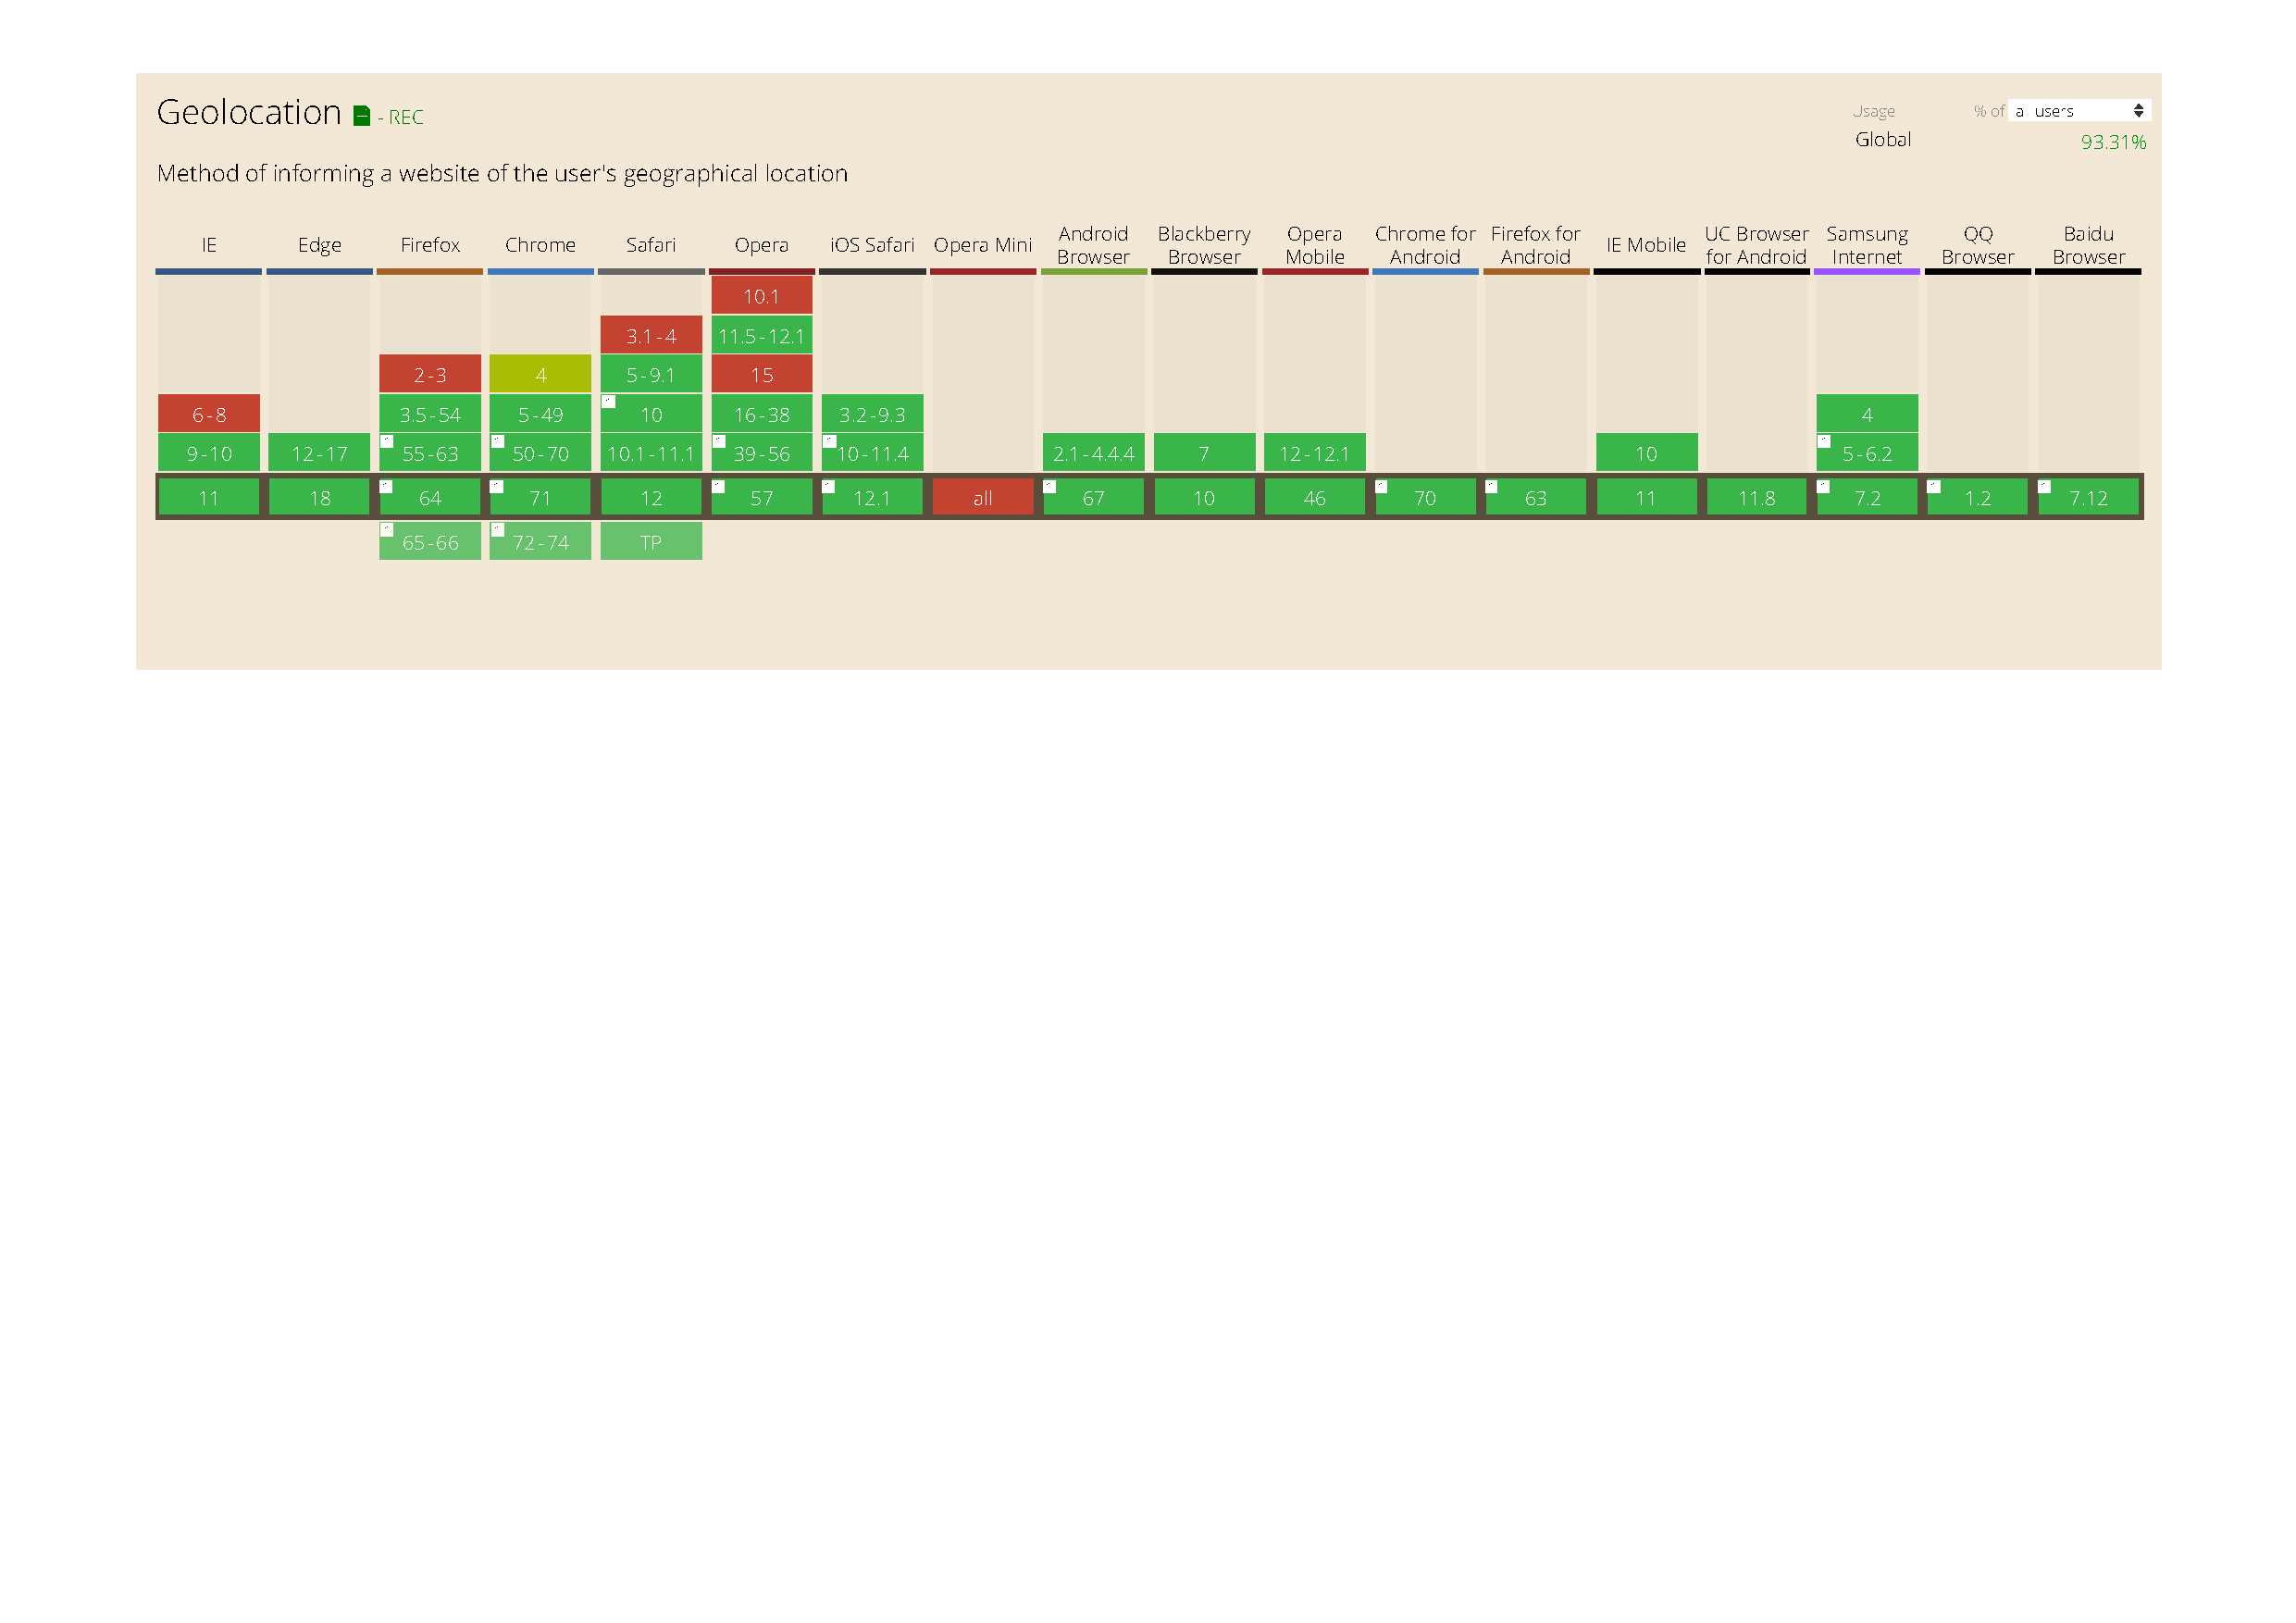
\includegraphics[width=\linewidth,trim=2.5cm 17.5cm 2.5cm 0cm]{caniuse.pdf}
  \caption{Browser support data for the Geolocation \textsc{api} (green means supported, red means not supported),
    data via \url{https://caniuse.com/\#feat=geolocation}}
  \label{fig:caniuse}
\end{figure*}

\subsection{\textsc{w3c} Geofencing \textsc{api}}

The \textsc{w3c} Geofencing \textsc{api}~\cite{kruisselbrink2017geofencing} specification
defined an \textsc{api} that should let Web applications set up geographic boundaries
around specific locations and then receive notifications when the hosting device
entered or left those areas, also referred to as geofences.
The Geolocation Working Group was chartered to define a~secure and privacy-sensitive interface
for using client-side location information in location-aware Web applications
and published an update to the Geolocation \textsc{api}~\cite{popescu2016geolocation}
specification as a~Recommendation excluding the geofencing feature,
which was being worked on in the context of the separate Geofencing \textsc{api} specification,
however, the work on it did not complete.
While it would be possible to implement something similar to geofencing using the Geolocation
\textsc{api} (as long as the application is in the foreground),
there were a~few differences that made the proposed \textsc{api} look like a~better choice,
quoting directly from the specification~\cite{kruisselbrink2017geofencing}:

\begin{quote}
``(1)~Because of the limited \textsc{api} surface of the Geofencing \textsc{api},
user agents can implement the \textsc{api} in a~more (power) efficient way
than could be achieved by regularly checking the current geographic position with the Geolocation
\textsc{api}.

(2)~The Geofencing \textsc{api} is built around Service Workers.
This makes it possible for a~webapp to receive notifications from the Geofencing \textsc{api}
even after the user has closed the webapp.''	
\end{quote}

\begin{lstlisting}[caption={Geofencing \textsc{api} (conceived example)},
  label=code:geofence, language=JavaScript, float=b] 
// On main page
navigator.serviceWorker
  .register('serviceworker.js')
  .then((swRegistration) => {
    let region = new CircularGeofenceRegion({
      name: 'myfence',
      latitude: 37.421999,
      longitude: -122.084015,
      radius: 1000
    });
    let options = {
      includePosition: true
    };
    swRegistration.geofencing.add(region, options)
      .then(
        // If more than just a name needs to be stored
        // with a geofence, now would be the time to
        // store this in some storage
        (geofence) => console.log(geofence.id),
        (error) => console.log(error)
      );
});

// In serviceworker.js
self.ongeofenceenter = (event) => {
  console.log(event.geofence.id);
  console.log(event.geofence.region.name);

  // If this is not a geofence of interest anymore,
  // remove it now
  if (event.geofence.region.name !== "myfence") {
    event.waitUntil(event.geofence.remove());
  }
};
\end{lstlisting}

It was not generally agreed on that Service Workers were the right technology
choice,\footnote{\url{https://www.w3.org/2014/10/27-28-geolocation-minutes.html\#day21}}
as they may be killed by the user agent at nearly any time,
which means one cannot expect \texttt{watchPosition()} to keep watching for extended periods,
and likewise the method \texttt{getCurrentPosition()} could only work if the position was already
available, but if it has to wait for a~\textsc{gps} update, the Service Worker is likely to be gone
by the time an answer comes back.

\section{Current Geolocation Efforts}

After having covered the significant milestones in the history of geolocation in the browser,
the second part of the paper introduces some of the current efforts, challenges,
and use cases in the field.

\subsection{Background Geolocation with Wake Locks}
\label{sec:wakelocks}

When a~device that has either of the two Geolocation \textsc{api} methods
\texttt{watchPosition()} or \texttt{getCurrentPosition()} running
goes into stand-by mode (colloquially ``goes to sleep''), or
when the browser window is backgrounded, location reporting stops soon thereafter.
This renders certain use cases like fitness run trackers or maps navigation
that both require background geolocation entirely impossible.
Wake Locks, initially introduced with the since discontinued
Firefox~\textsc{os}~\cite{francis2017firefoxos}, provided
a~way\footnote{\url{https://developer.mozilla.org/en-US/docs/Archive/B2G_OS/API/Wake_Lock_API/Keeping_the_geolocation_on_when_the_application_is_invisible}}
to prevent the system from sleeping and to keep certain services running
when the developer wanted to keep an invisible application continuing to use \textsc{gps}.
This could be done by requesting a~\texttt{MozWakeLock} of the type \texttt{"gps"}
and using it together with \texttt{watchPosition()}.
App developers needed to be responsible and think carefully about
whether they needed to keep the geolocation service on or not.
The risk of claiming the lock was (and still is) that users may forget to close the app
when they were done using it, which inevitably results in significantly increased battery use,
apart from the privacy implications of potentially inadvertently continuing to share one's location.

Work on the concept of Wake Locks has been resumed in the form of the \textsc{w3c}
Wake Lock specification~\cite{bogdanovich2017wakelock}.
With the at the time of writing implemented version of the specification,
Wake Locks of the type \texttt{"system"}
(currently there is no type \texttt{"gps"}) can be used together with \texttt{watchPosition()}.
\autoref{code:wakelock} shows the relevant code excerpts of a~Web application
called ``Where Am~I'', depicted in \autoref{fig:wakelock}, that implements this,
simulating a~simple run tracker that works with the device screen off while the user runs.
The accompanying app ``There Am~I''\footnote{\url{https://whereami.glitch.me/} and
\url{https://thereami.glitch.me/}} can be used to visualize users.

\begin{lstlisting}[caption={Using the Wake Lock \textsc{api} for background geolocation tracking},
  label=code:wakelock, language=JavaScript, float=t] 
try {
  wakeLockObj = await navigator.getWakeLock('system');
  wakeLockObj.addEventListener('activechange', () => {
    wakelock.textContent =
        `The ${wakeLockObj.type} wake lock is ${
        wakeLockObj.active ? 'active' : 'not active'}.`;
  });
} catch (err) {
  console.error('Could not obtain wake lock', err);
}

const toggleWakeLock = () => {
  if (wakeLockRequest) {
    wakeLockRequest.cancel();
    wakeLockRequest = null;      
    return;
  }
  wakeLockRequest = wakeLockObj.createRequest();
};
    
const startTracking = () => {  
  id = navigator.geolocation.watchPosition(success,
      error, opt);  
};

trackButton.addEventListener('click', () => {
  toggleWakeLock();    
  if (id) stopTracking();
  else startTracking();
});
\end{lstlisting}

\begin{figure}[h]
  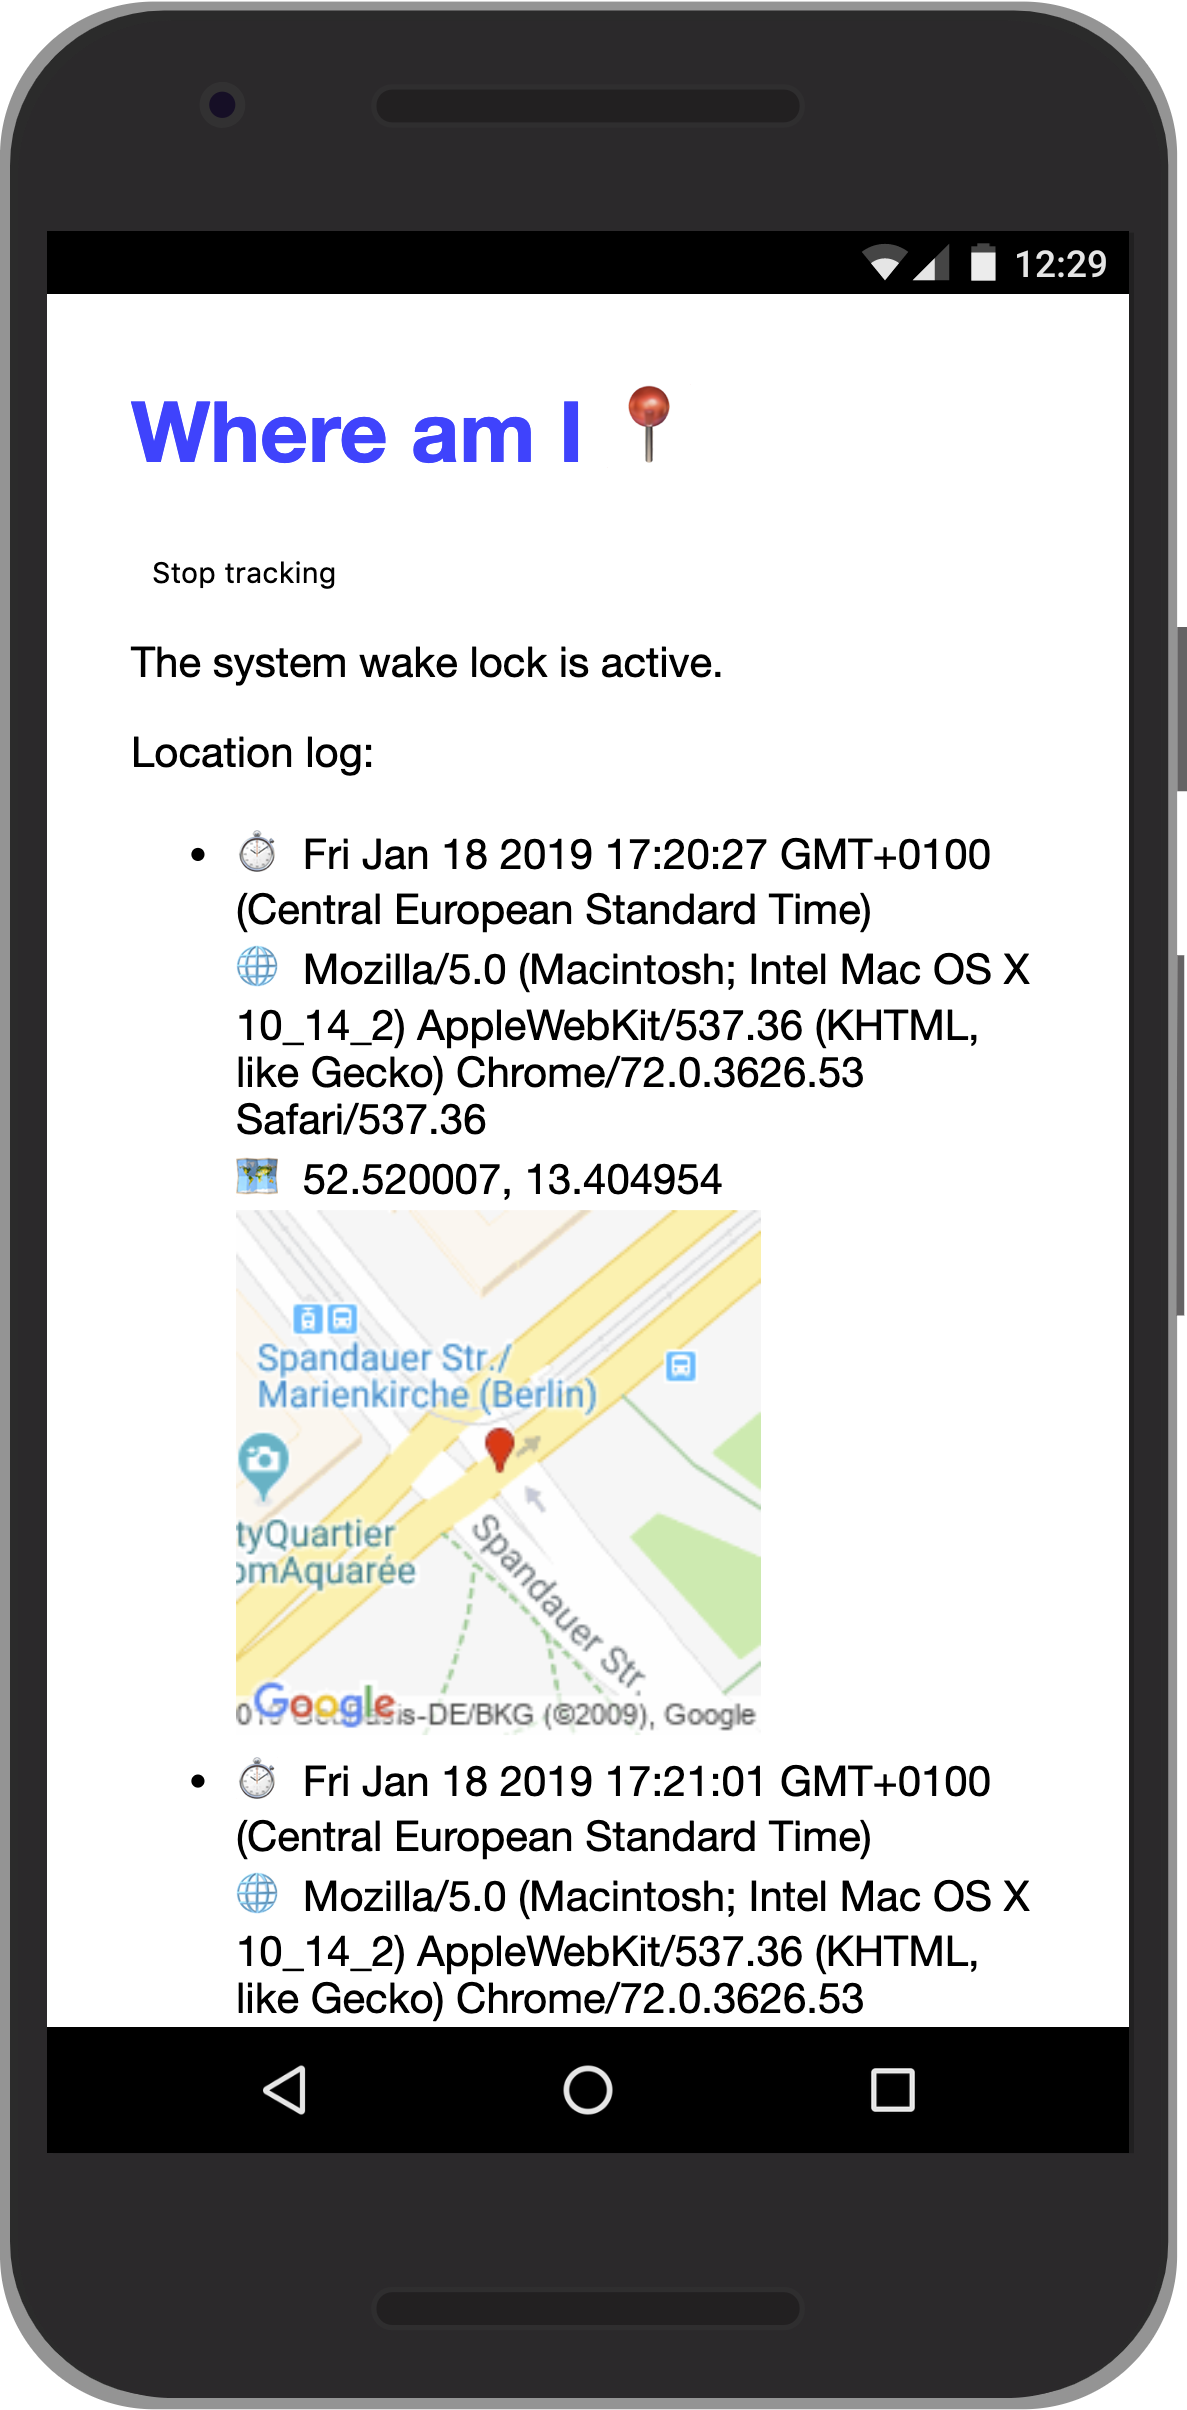
\includegraphics[width=0.45\columnwidth]{whereami.png}
  \caption{Web app ``Where Am~I''
    with Wake Lock for background location tracking (\url{https://whereami.glitch.me/})}
  \label{fig:wakelock}  
\end{figure}

\subsection{Geolocation Sensor}

The \textsc{w3c} Geolocation Sensor specification~\cite{kostiainen2018geolocation}
extends the \texttt{Sensor} interface defined in the
\textsc{w3c} Generic Sensor \textsc{api}~\cite{waldron2018genericsensor}
to in turn define the new \texttt{GeolocationSensor} interface
for obtaining the geolocation of the hosting device.
The Generic Sensor \textsc{api} is a~set of interfaces that expose sensor devices to the Web
platform. It consists of the base \texttt{Sensor} interface and a~set of concrete sensor classes
(for example \texttt{GeolocationSensor}, \texttt{AmbientLightSensor}, \texttt{Accelerometer},
\textit{etc.}) built on top.
Having a~base interface simplifies the implementation and specification process for the concrete
sensor classes. The core functionality is specified by the base interface, and
\texttt{GeolocationSensor} merely extends it with a~tiny set of additional attributes and methods.
The feature set of \texttt{GeolocationSensor} is similar
to that of the Geolocation \textsc{api}~\cite{raskin2010geolocation},
but it is surfaced through a~modern \textsc{api} that is consistent across contemporary Sensor
\textsc{api}s, improves security and privacy, and is extensible.
The \textsc{api} aims to be
polyfillable\footnote{\url{https://github.com/w3c/sensors/blob/master/polyfills/geolocation.js}}
on top of the existing Geolocation \textsc{api}.
As all recent \textsc{api}s, instead of callbacks, Geolocation Sensor
uses promises for ``one-shot'' or ``one-and-done''
operations~\cite{denicola2018tag}.

Unlike with the previous Geolocation \textsc{api}, the Geolocation Sensor \textsc{api}
does not have dedicated callbacks for
``one-shot'' versus continuous location
requests,\footnote{\texttt{GeolocationSensor} does have a~dedicate static operation
\texttt{read()} for ``one-shot''}
but instead fires an event according to a~frequency (in Hertz) that is used
to calculate the requested sampling frequency for the associated platform sensor
and to define the upper bound of the reporting frequency for the \texttt{GeolocationSensor}
object.
\autoref{code:geolocationsensor} shows the \textsc{api} in practice,
however, running it requires a~polyfill, as currently there is no native implementation.

\begin{lstlisting}[caption={Geolocation Sensor \textsc{api}},
  label=code:geolocationsensor, language=JavaScript, float=t] 
// Get a new geolocation reading every second
const geo = new GeolocationSensor({frequency: 1});
geo.start();

geo.onreading = () => console.log(
    `lat: ${geo.latitude}, long: ${geo.longitude}`);

geo.onerror = event => console.error(
    event.error.name, event.error.message);

// Get a one-shot geolocation reading
GeolocationSensor.read()
  .then(geo => console.log(
      `lat: ${geo.latitude}, long: ${geo.longitude}`))
  .catch(error => console.error(error.name));
\end{lstlisting}

\section{Geolocation Privacy}

Security and privacy issues for location-based services and geolocation-capable applications
often revolve around designing a user interface such that users are informed
about what an application is doing and have the ability to accept or decline~\cite{doty2010gpa}.
Use cases like background geolocation or geofencing
demand for a~thorough re-evaluation of privacy-related questions.
Similarly, some of the requirements that today we take for granted
just did not exist when the Geolocation \textsc{api} was designed,
like the strict requirement to be on a~secure connection for using modern
\textsc{api}s.\footnote{Internet Explorer up to version~11 even warned its users
``You are about to view pages over a secure connection''
when they navigated to a~site that used the \textsc{https} protocol.}

\subsection{Insecure Origin Usage of Geolocation}

As the Web platform is extended to enable more useful and powerful applications,
it becomes increasingly important to ensure that the features
which enable those applications are enabled only in contexts
which meet a~minimum security level.
The Secure Contexts specification~\cite{west2016securecontexts}
describes threat models for feature abuse on the Web as follows:

\begin{quote}
``Granting permissions to unauthenticated origins is, in the presence of a~network attacker,
equivalent to granting the permissions to any origin.
The state of the Internet is such that we must indeed assume that a~network attacker is present.
Generally, network attackers fall into two classes: passive and active.

\textbf{1. Passive Network Attacker:} A~`Passive Network Attacker' is a~party
who is able to observe traffic flows but who lacks the ability
or chooses not to modify traffic at the layers which this specification is concerned with. [\ldots]

\textbf{2. Active Network Attacker:} An `Active Network Attacker' has all the capabilities
of a~`Passive Network Attacker' and is additionally able to modify, block or replay
any data transiting the network.
These capabilities are available to potential adversaries at many levels of capability,
from compromised devices offering or simply participating in public wireless networks,
to Internet Service Providers indirectly introducing security and privacy vulnerabilities [\ldots],
to parties with direct intent to compromise security or privacy who are able to target individual
users, organizations or even entire populations.''
\end{quote}

In a~rare case of breaking backwards compatibility and after a~careful risk analysis,
the concepts in~\cite{west2016securecontexts} were applied
to features that had already shipped in browsers
and which did not meet the---new, not present at the time---requirements.
Specifically, geolocation support was removed on insecure origins,
motivated by the large privacy risk for end users of even passive attackers
sniffing geolocation obtained from this \textsc{api}.

\subsection{Feature Policy Integration}

Feature Policy~\cite{clelland2019featurepolicy} defines a~mechanism that allows developers
to selectively enable and disable use of various browser features and \textsc{api}s.
The Feature Policy integration in the Generic Sensor \textsc{api}
is used to control access to sensors data for a~frame.
By default the \texttt{Sensor} objects (and therefore the \texttt{GeolocationSensor})
can be created only within a~main frame or same-origin subframes,
thus preventing cross-origin iframes from unsanctioned reading of sensor data.
This default behavior can be modified by explicitly enabling or disabling
of the corresponding policy-controlled features.
\autoref{code:featurepolicy} illustrates granting geolocation data access to a~cross-origin iframe,
meaning that now \texttt{GeolocationSensor} objects can be created there.

\begin{lstlisting}[caption={Allowing an iframe to use \texttt{GeolocationSensor}},
  label=code:featurepolicy, language=HTML, float=h] 
<iframe src="https://3rd-party.com" allow="geolocation">
\end{lstlisting}

\subsection{Focused Area and Visibility State}
\label{sec:focusandvisibility}

Sensor readings are only available for active documents whose origin is same origin-domain
with the currently focused area document and whose visibility state is \texttt{"visible"}.
This is done in order to mitigate the risk of a~skimming attack
against the browsing context containing an element which has gained focus,
for example when the user carries out an in-game purchase using a~third party payment service
from within an iframe.
Similar to \autoref{sec:wakelocks}, these to be re-evaluated constraints
currently limit use cases like fitness run trackers
or maps navigation that require sensor readings in potentially non-active, non-visible documents,
for example while the user chooses a~music track to accompany their run or drive.

\subsection{Permissions and Privacy Policy}

Access to sensor readings are controlled by the \textsc{w3c} Permissions
\textsc{api}~\cite{lamouri2017permissions}.
User agents use a~number of criteria to grant access to the readings.
Note that while access to some sensors can be granted without prompting the user,
\texttt{GeolocationSensor} always requires a~prompt.
\autoref{code:prompt} shows the permissions flow that is required before any readings.
In contrast, with the legacy Geolocation \textsc{api}, the user agent prompts the user automatically
upon the first time they try to use either of \texttt{watchPosition()} or
\texttt{getCurrentPosition()}.

\begin{lstlisting}[caption={Asking for permission to use \texttt{GeolocationSensor}},
  label=code:prompt, language=JavaScript, float=h] 
navigator.permissions.query({name: "geolocation"})
  .then(({state}) => {
    switch (state) {
      case "granted":
        showLocalNewsWithGeolocation();
        break;
      case "prompt":
        showButtonToEnableLocalNews();
        break;
      default:        
        break; // Don't do anything if permission denied
    }
  });
\end{lstlisting}

The current permission prompt has the options to allow or to block
the location access request (or, for what it is worth, to ignore it by closing the dialog).
Interestingly, Raskin envisioned~\cite{raskin2010geolocation} a~far more detailed permissions
dialog, depicted in \autoref{fig:promptraskin}, which had granular levels of permitted access,
for example, to limit the granularity to city or state level.
However, this was never implemented, as despite being fully investigated, it was found to be nearly
impossible to implement ``fuzzing'' of location data~\cite{thomson2011obscuring}.

\begin{figure}[h]
  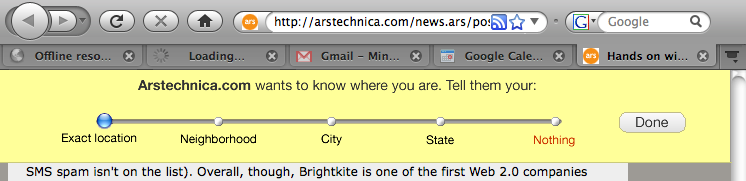
\includegraphics[width=0.85\columnwidth]{mockup-prompt.png}
  \caption{Aza Raskin's security prompt mock-up~\cite{raskin2010geolocation}}
  \label{fig:promptraskin}
\end{figure}

With use cases like run trackers, it would additionally be of interest
to limit access to background geolocation data to a~given time period,
for example, the duration of a~one hour run.
This is currently not possible, and the Permissions specification~\cite{lamouri2017permissions}
is intentionally vague regarding the storage of permissions,
leading to some user agents (\textit{e.g.}, Chrome) to persist decisions,
others (\textit{e.g.}, mobile Safari) to ask every time,
and yet others (\textit{e.g.}, desktop Safari or Firefox)
to optionally remember them (time-limited for Safari).

A~notable privacy discussion was happening between the \textsc{ietf} \textsc{geopriv}
and the \textsc{w3c} Geolocation Working Groups around the question of whether or not
a~privacy policy should be included in the Geolocation \textsc{api} itself,
or rather be addressed as a~set of recommendations and requirements in the specification.
The Geolocation Working Group
concluded\footnote{\url{https://www.ietf.org/lib/dt/documents/LIAISON/file727.txt}}
that privacy protection was better handled
as part of a~more generic privacy and security framework for device access.
Privacy and security threats now take a~significant amount of space
in the Generic Sensor specification~\cite{waldron2018genericsensor}.

\section{Future Work and Conclusion}

Future work will happen in several areas and touch upon both technological
as well as user privacy related aspects.
In the following paragraphs, we present some of them,
but note that especially the permission aspects reach a~lot further than geolocation.

We will continue our experiments with Wake Locks~\cite{steiner2018wakelock}
and how they can interact with Geolocation Sensor,
with a~special focus on sensor readings in non-focused and non-visible states
(\autoref{sec:focusandvisibility}).
Further, after having explored use cases around background geolocation
and geofencing~\cite{kostiainen2018geolocation} in more detail,
we will resume our work on Geofencing~\cite{kruisselbrink2017geofencing}
and investigate integration of this feature with Geolocation
Sensor~\cite{kostiainen2018geolocation}, possibly via the extensibility mechanism defined in Service
Workers~\cite{russell2017serviceworkers}
that makes them extensible from other specifications through a~functional event
by extending the \texttt{ExtendableEvent} interface.

User privacy is central to all sensor readings, and particularly to geolocation.
As outlined in \autoref{sec:googlegears}, from the start it was a~major concern
and especially with new background geolocation and geofencing use cases,
it remains an issue of high importance.
In~\cite{russell2018permissions}, Russell and Nattestad have explored permission dialog
abuse, annoyance, and fatigue of users; and according to their opinion (which we support),
``today's permissions model and \textsc{api} surface area should be heavily revised
[\ldots] to enable more flexible permission policies'' in a~more uniform
Permissions \textsc{api}~\cite{lamouri2017permissions}.
Some ideas include supporting both time-limited as well as one-off requests and permission grants,
but also extending Web Application Manifest~\cite{caceres2018manifest}
to allow sites to identify to the runtime a~maximum set of permissions,
and turn down permission requests not explicitly included in the Web Application Manifest,
with installability~\cite{caceres2018manifest} of Web apps potentially considered an additional
trust factor.

Concluding, in this paper we have first provided an overview
of the historical development of geolocation in the browser,
and given an outlook on current and future efforts, challenges, and use cases in the field.
The importance of user privacy is ever-increasing, and in our work on geolocation,
background geolocation, and geofencing,
we keep privacy as a~top priority.
While many privacy concerns such as unsanctioned third-party access and fingerprinting
can now be mitigated by technical measures, we continue to work with the privacy research community
to ensure the Web remains a~both capable and safe platform today and in the future
by carefully assessing every new proposed feature for possible privacy threats.

\section*{Acknowledgements}

We are thankful to \textit{Doug Turner} for his invaluable help
with getting the historical facts right and to \textit{Alex Russell} for reviewing the paper.

\bibliographystyle{ACM-Reference-Format}
\balance 
\bibliography{bibliography}

\end{document}
